\documentclass[dvipdfmx,12pt,a4paper]{jreport}
	\usepackage{geometry}
    \usepackage{pdfpages}
    \usepackage{graphicx}
    \usepackage{newtxmath}
    \usepackage{array}
    \usepackage{siunitx}
    \usepackage{url}
    \usepackage{amsmath}
    \usepackage{comment}
    \usepackage{amsfonts}
    \usepackage{here}
    \geometry{left=20mm,right=20mm,top=25mm,bottom=25mm} %geometry:余白設定
    \renewcommand{\bibname}{参考文献}
    %\renewcommand{\figurename}{Fig.}
    %\renewcommand{\tablename}{Tab.}
    \makeatletter
    \DeclareRobustCommand\cite{\unskip
    	\@ifnextchar[{\@tempswatrue\@citex}{\@tempswafalse\@citex[]}}
    \def\@cite#1#2{$^{\hbox{\scriptsize{[#1\if@tempswa , #2\fi}]}}$}
    \def\@biblabel#1{[#1]}
    \makeatother
    
    \graphicspath{{./graphics/}} %図のディレクトリを設定.フォルダの場所によって先頭' . 'の数を変える.
\begin{document}
	\begin{titlepage}
		
		\begin{center}
			
			\vspace{20truept}
			{\LARGE 2022年度}\\
			\vspace{15truept}
			{\LARGE 修士論文}
			
			\vspace{50truept}
			
			{\Huge Silk Fibroin Filmの圧電性向上の研究}\\
			\vspace{10truept}
			
			\vspace*{280truept}
			
			{\LARGE 1521516}\\
			\vspace{5truept}
			
			{\LARGE 金木 進}\\
			\vspace{60truept}
			
			{\LARGE 2023年3月}
			\vspace{30truept}
			
			{\LARGE 東京理科大学}\\
			\vspace{15truept}
			
			{\LARGE 理学研究科 応用物理学専攻}\\
			\vspace{15truept}
			
			{\LARGE 中嶋研究室}\\
			
		\end{center}
		
		
	\end{titlepage}
  \thispagestyle{empty}
	\clearpage
\addtocounter{page}{0}
\tableofcontents
  \chapter{序論}
		\section{研究背景}
		\section{研究の目的}
	\chapter{原理}
		\section{圧電基本式と電気機械結合係数}
		圧電体には正圧電効果と逆圧電効果という性質が存在する。
		生じた歪みに対して、応力と電場の寄与がある。
		さらに生じた電束密度に対しても電場と歪みの二つの寄与がある。
		これらを式にまとめると
				\begin{eqnarray}
					\begin{cases}
						\delta S=\frac{\partial S}{\partial T}\delta T + \frac{\partial S}{\partial E} \delta E 
						= s^{E}\delta T+d \delta E & \\
						\delta D=\frac{\partial D}{\partial T}\delta T + \frac{\partial D}{\partial E}\delta E 
						= d \delta T+\varepsilon^T \delta E  &
					\end{cases}
					\label{圧電d形式1}
				\end{eqnarray}
			となる。実際の試料は1軸方向、2軸方向、3軸方向のみだけでなく、
			せん断歪みを考慮する必要があり、テンソル形式で記述される。
			ここで、$\delta S\rightarrow S, \delta T\rightarrow T,
			\delta E\rightarrow E, \delta D\rightarrow D$とし、テンソル行列を$\left[ \right]$で表すと
			式\ref{圧電d形式1}は
			\begin{equation}
				\begin{cases}
					\left[S\right]=\left[s^E\right]\left[T\right]+\left[d_t\right]\left[E\right]& \\
					\left[D\right]=\left[d\right]\left[T\right]+\left[\varepsilon^T\right]\left[E\right]
				\end{cases}
				\label{圧電d形式2}
			\end{equation}
			となり、これを圧電d形式と呼ぶ。
			式\ref{圧電d形式2}をテンソルの要素も含めて記述すると
			\begin{equation}
				\begin{cases}
				\left(
				\begin{array}{c}
					S_1 \\
					S_2 \\
					S_3 \\
					S_4 \\
					S_5 \\
					S_6 
				\end{array}
				\right)=\left(
				\begin{array}{cccccc}
				s^E_{11} & s^E_{12} & s^E_{13} & 0 & 0 & 0 \\
				s^E_{21} & s^E_{22} & s^E_{23} & 0 & 0 & 0 \\
				s^E_{13} & s^E_{32} & s^E_{33} & 0 & 0 & 0 \\
				0 & 0 & 0 & s^E_{44} & 0 & 0 \\
				0 & 0 & 0 & 0 & s^E_{44} & 0 \\
				0 & 0 & 0 & 0 & 0 & s^E_{66} 
				\end{array}
				\right)
				\left(
				\begin{array}{c}
					T_1 \\
					T_2 \\
					T_3 \\
					T_4 \\
					T_5 \\
					T_6 
				\end{array}
				\right)+
				\left(
				\begin{array}{ccc}
					0&0	&d_{31} \\
					0&0	&d_{31} \\
					0&0	&d_{33} \\
					0&d_{15}&0 \\
					d_{15}&0&0 \\
					0&0	&0 
				\end{array}
				\right)
				\left(
				\begin{array}{c}
					E_1 \\
					E_2 \\
					E_3 \\
				\end{array}
				\right) & \\
				\left(
				\begin{array}{c}
					D_1 \\
					D_2 \\
					D_3
				\end{array}\right)=\left(
				\begin{array}{cccccc}
					0&0&0&0&d_{15}&0 \\
					0&0&0&d_{15}&0&0 \\
					d_{31}&d_{31}&d_{33}&0&0&0
				\end{array}\right)
				\left(
				\begin{array}{c}
					T_1 \\
					T_2 \\
					T_3 \\
					T_4 \\
					T_5 \\
					T_6 
				\end{array}
				\right)+\left(
				\begin{array}{ccc}
					\varepsilon^T_{11}&0&0 \\
					0&\varepsilon^T_{11}&0 \\
					0&0&\varepsilon^T_{33}
				\end{array}\right)
				\left(
				\begin{array}{c}
					E_1 \\
					E_2 \\
					E_3 \\
				\end{array}\right)
				\end{cases}
			\end{equation}
			となる。また、$s^E_{66}=2\left(s^E_{11}-s^E_{12}\right)$である。
			式\ref{圧電d形式2}を式変形すると
			\begin{equation}
				\begin{cases}
				\left[T\right]=\left[c^E\right]\left[S\right]-\left[e_t\right]\left[E\right] & \\
				\left[D\right]=\left[e\right]\left[S\right]+\left[\varepsilon^S\right]\left[E\right]
				\end{cases}
				\label{圧電e形式}
			\end{equation}
			\begin{equation}
				\begin{cases}
					\left[S\right]=\left[s^D\right]\left[T\right]-\left[g_t\right]\left[D\right] & \\
					\left[E\right]=-\left[g\right]\left[T\right]+\left[\beta^T\right]\left[D\right]
				\end{cases}
				\label{圧電g形式}
			\end{equation}
			\begin{equation}
				\begin{cases}
					\left[T\right]=\left[c^D\right]\left[S\right]-\left[h_t\right]\left[D\right] & \\
					\left[E\right]=-\left[h\right]\left[S\right]+\left[\beta^s\right]\left[D\right]
				\end{cases}
				\label{圧電h形式}
			\end{equation}
			の三式を導け、それぞれ式\ref{圧電e形式}を圧電e形式, 
			式\ref{圧電g形式}を圧電g形式, 式\ref{圧電h形式}を圧電h形式と呼ぶ。応力$T$, 電場$E$, 歪み$S$, 電束密度$D$の係数である$[d],[e],[g],[h]$ではそれぞれ、
			\begin{equation}
				d_{ij}=\left(\frac{\partial D_i}{\partial T_j}\right)_E=\left(\frac{\partial S_j}{\partial E_i}\right)_T
			\end{equation}
			\begin{equation}
				e_{ij}=\left(\frac{\partial D_i}{\partial S_j}\right)_E=-\left(\frac{\partial T_j}{\partial E_i}\right)_S
			\end{equation} 
			\begin{equation}
				g_{ij}=-\left(\frac{\partial E_i}{\partial T_j}\right)_D=\left(\frac{\partial S_j}{\partial D_i}\right)_T
			\end{equation}
			\begin{equation}
				h_{ij}=-\left(\frac{\partial E_i}{\partial S_j}\right)_D=-\left(\frac{\partial T_j}{\partial D_i}\right)_S
			\end{equation}
			で定義される。また、それぞれの圧電定数間には弾性コンプライアンス$s$、
			誘電率$\varepsilon$を介して以下の関係がある。
			\begin{equation}
				d = e s
			\end{equation}
			\begin{equation}
				g = h s
			\end{equation}
			\begin{equation}
				d = \varepsilon g
			\end{equation}
			\begin{equation}
				e = \varepsilon h
			\end{equation}

			圧電定数と同様に、圧電効果を示す定数として電気機械結合係数$k$がある。
			電気機械結合係数$k$は電気的エネルギーと機械的エネルギーの変換を表す係数であり、
			式\ref{電気機械結合係数の定義}のように与えた電気エネルギーと生じた機械エネルギー、
			あるいは与えた機械的エネルギーと生じた電気的エネルギーの比の平方根で定義される。
			\begin{equation}
			k^2=\frac{\mbox{出力機械的エネルギー}}{\mbox{入力電気的エネルギー}}=
			\frac{\mbox{出力電気的エネルギー}}{\mbox{入力機械的エネルギー}}
			\label{電気機械結合係数の定義}
			\end{equation}
			また、電気機械結合係数は$k$は$k_{31}, k_{33}$の様に、
			電場方向と機械入出力方向を示す二つの下付き文字で表現される。
			表\ref{圧電材料}に代表的な圧電材料であるPZTとPVDFの物性値をまとめた。
			\begin{table}[h]
				\centering
				\caption{PZTとPVDFの物性値}
				\label{圧電材料}
				\begin{tabular}{c|ccccc}\hline
					材料&弾性率[N/m$^2$]&比誘電率$\varepsilon/\varepsilon_0$&$d_{31}$[pC/N]&$g_{31}$[Vm/N]&電気機械結合係数$k_{31}$ \\ \hline \hline
					PZT&83.3&1200&110&0.01&0.31 \\
					PVDF&3.0&13&20&0.17&0.10 \\ 
					水晶&77&4.5&2&0.05&0.09 \\
					VDCN/VAc&4.5&5&6&0.13&0.06 \\ 
					VDCN/MMA&4.5&5&0.3&0.007&0.003 \\ \hline
				\end{tabular} 
			\end{table}
	\chapter{実験手法}
		\section{試料作製方法}
		\section{評価方法}
			\subsection{$\theta - 2\theta$測定(XRD)}
			\subsection{Pole Figure測定(XRD)}
			
			\newpage

			\subsection{原子間力顕微鏡(AFM), 圧電応答顕微鏡(PFM)}
			原子間力顕微鏡(AFM)、圧電応答顕微鏡(PFM)はどちらも走査型プローブ顕微鏡(SPM)に属する。
			走査型プローブ顕微鏡(SPM)とは、微小な深針(カンチレバー)で試料をなぞり、
			その形状や物性を観察、計測する顕微鏡の総称である。図\ref{SPM}, \ref{cantilever_photo_detector}
			にSPMの基本構成を示す。SPMに属する顕微鏡は図\ref{SPM}のように
			カンチレバーを試料表面に接触または接近させて、走査中に生じる試料のある物理量の変化を検出する。
			本研究にて用いるSPMは原子間力顕微鏡(AFM)と圧電応答顕微鏡(PFM)のみである。
			この二つにおいては、図\ref{cantilever_photo_detector}のようにそれぞれの物理量変化
			によってカンチレバーがたわみ、そのカンチレバーに照射したレーザーの変位を
			フォトディテクターで計測し、測定対象の物理量変化を測定する。
			つまり、レーザーの変位から物質表面の物性変化をみる。
			原子間力顕微鏡(AFM)はカンチレバーと試料間に生じる原子間力を検出し
			試料表面画像を取得する。圧電応答顕微鏡(PFM)は試料の逆圧電効果に
			よる表面の歪みをカンチレバーの変位として取得し画像化する。
			\begin{figure}[h]
				\centering
				\begin{minipage}{0.45\hsize}
					\centering
					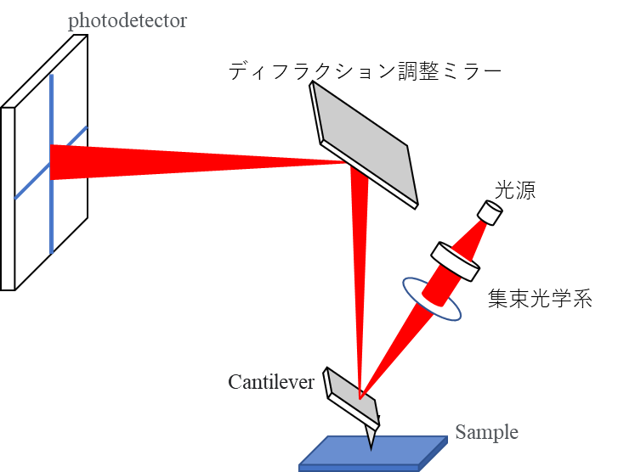
\includegraphics[width=\linewidth]{SPM.png}
					\caption{走査型顕微鏡(SPM)の光学系}
					\label{SPM}
				\end{minipage}
				\begin{minipage}{0.45\hsize}
					\centering
					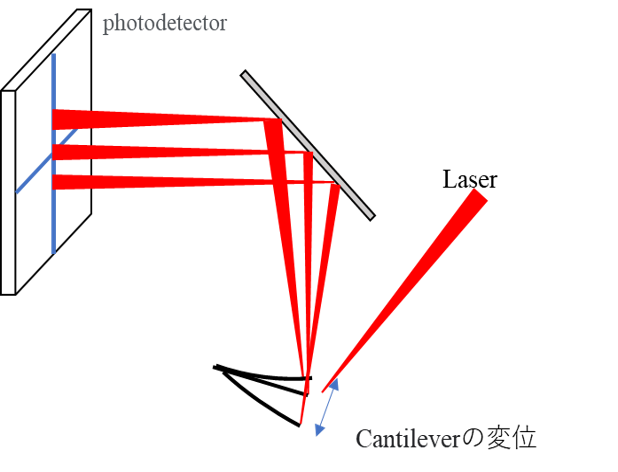
\includegraphics[width=\linewidth]{SPM2.png}
					\caption{CantileverとPhotodetectorの関係}
					\label{cantilever_photo_detector}
				\end{minipage}
			\end{figure}
				\subsubsection{AFM(Atomic Force Microscopy)}
				\begin{figure}[h]
					\centering
					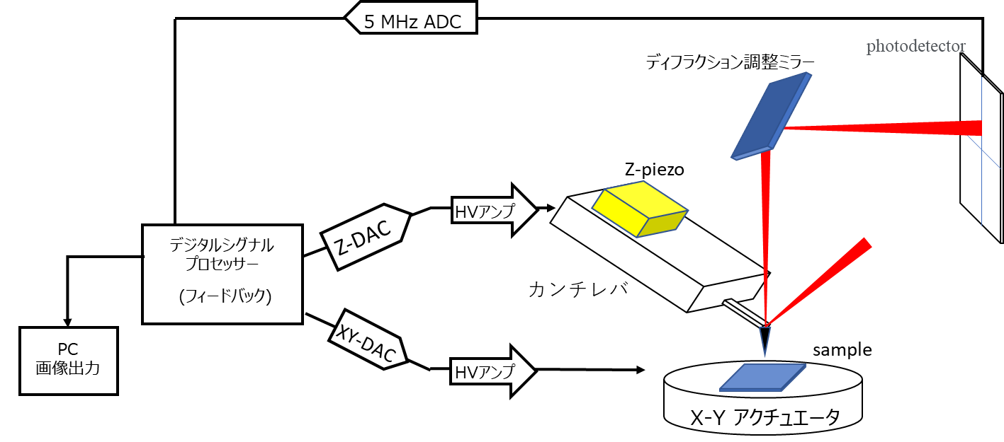
\includegraphics[width=0.8\linewidth]{AFM.png}
					\caption{AFMの信号模式図}
					\label{stracture_of_AFM}
				\end{figure}
				図\ref{stracture_of_AFM}はAFMの信号模式図である。AFMの測定手法にはタッピングモード(ACモード)
				とコンタクトモード(DCモード)がある。タッピングモードは、カンチレバーを内部に存在する圧電素子を用いて
				共振周波数で振動させ、試料表面を断続的に接触させながら走査する。測定対象の表面形状からカンチレバーの振動振幅が変動し、
				画像化する。正確にはカンチレバーを試料表面に近づけると原子間力を検出し、
				この瞬間カンチレバーの振動振幅は小さくなる。この振動振幅の変位をレーザーの変位として取得し、
				この変位分だけ元に戻すようにフィードバックをかけ、Z軸方向をZピエゾで調整する。このZピエゾの変位を画像化し、表面像を得る。
				コンタクトモードはタッピングモードと異なり、
				カンチレバーを振動させずに静的な状態で試料に常に接触させながら試料表面を走査し、
				表面の凹凸に対応したカンチレバーのたわみをレーザーの変位としてフォトディテクターから検出する。
				このレーザーの変位を一定にするようにZピエゾを用いて、フィードバック制御を行う。そのZピエゾの変位を表面形状として画像化する。
				本研究において、AFMを用いた計測はカンチレバーの消耗の観点からタッピングモードで行った。
				\subsubsection{PFM(Piezoresponse Force Microscopy)}
				走査型プローブ顕微鏡(Scanning Prob Microscope, SPM)の一種として圧電応答顕微鏡(Piezoresponse Force Microscopy, PFM)がある。
				圧電応答顕微鏡(PFM)は試料の逆圧電効果による表面の歪みをカンチレバーの変位として取得し画像化する顕微鏡である。
				図\ref{PFMの概念図}のように試料片面基板からカンチレバー間で交流電場を印加する。
				このとき試料の分極方向に依存して、電場の変化に対応した歪みが試料に生じる。
				その歪の大きさはカンチレバーの変位の大きさとして現れ、
				Amplitude像として取得できる。
				\begin{figure}[h]
					\centering
					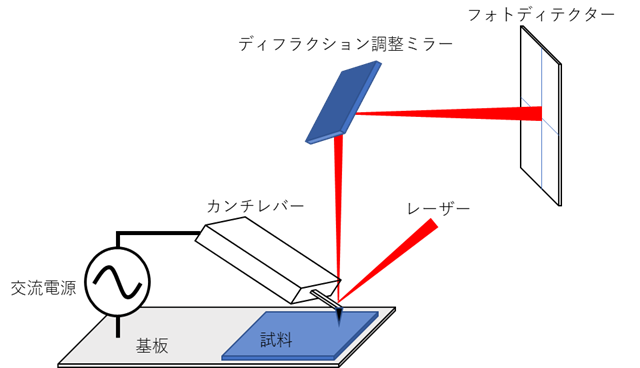
\includegraphics{PFM.png}
					\caption{PFMの概念図}
					\label{PFMの概念図}
				\end{figure}
				\\
				また、図\ref{PFM_phaseの概念図}のように交流電場に対応した試料の歪み方向は試料中の分極方向に依存しているため、
				この分極方向を交流電場と歪みの位相差から解析し、Phase像として取得できる。
				\begin{figure}[h]
					\centering
					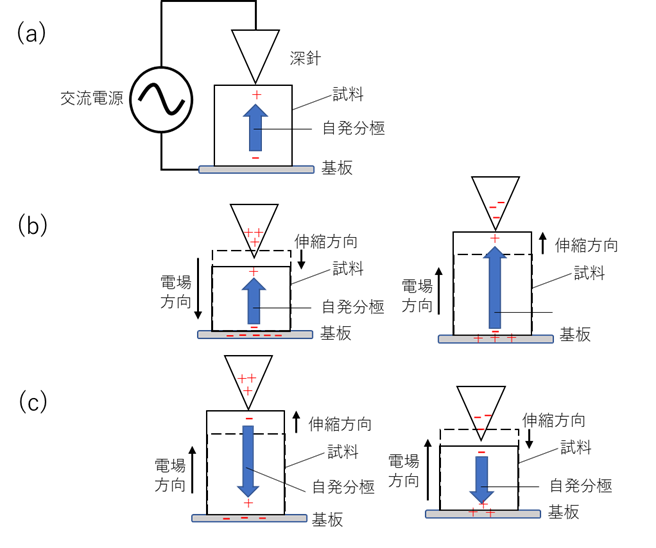
\includegraphics{PFM_phase.png}
					\caption{PFMのPhase像概念図。(a):電場E=0,(b):交流電場と試料の伸縮方向が同位相であるときの自発分極方向,(c):交流電場と試料の伸縮方向が逆位相であるときの自発分極方向}
					\label{PFM_phaseの概念図}
				\end{figure}
				PFMはカンチレバーを試料上に接触させ走査するコンタクトモードで行われる。
				カンチレバーと試料からの相互作用を加味した共振周波数、
				コンタクト周波数でカンチレバーを振動させることで、
				その振動振幅の変化から、より高精度に圧電応答を観察できるようになっている。
				しかし、そのコンタクト周波数は走査中一定に保たれているわけではない。
				なぜならば、走査中の試料表面の形状変化によるカンチレバーの接触面積の違いがコンタクト周波数をシフトさせる要因になる。
				コンタクト周波数のシフトにより、圧電応答によるカンチレバーのたわみ変化の大きさと走査中における試料表面の形状変化によるカンチレバーのたわみ変化がクロストークしてしまい、
				正確な圧電応答や表面像を取得できなくなる。よって測定材料は測定前に表面を平らにする必要がある。
				
				図\ref{PFM_phaseの概念図}は垂直方向のみでの議論である。しかし、図\ref{PFMの概念図}におけるフォトディテクターから分かる通り、
				図\ref{面内と垂直の概念図}の通り、試料の面内方向の圧電性の評価も可能である。本研究においてはずり圧電の評価にて使用した。
				\begin{figure}[h]
					\centering
					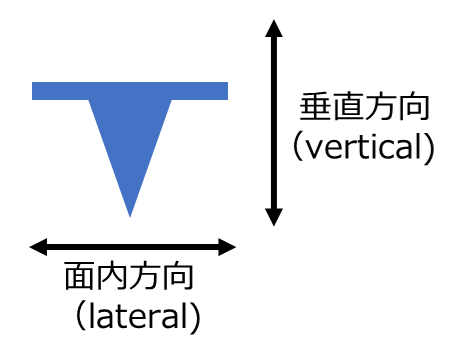
\includegraphics{lateral_vertical.png}
					\caption{カンチレバーにおける面内方向(Lateral)と垂直方向(Vertical)の関係}
					\label{面内と垂直の概念図}
				\end{figure}
				\newpage
				生体材料の一つであるコラーゲンの圧電行列は以下の通りである。
				\begin{equation}
					\left(
				\begin{array}{cccccc}
					0&0&0&d_{14}&d_{15}&0 \\
					0&0&0&d_{15}&-d_{14}&0 \\
					d_{31}&d_{31}&d_{33}&0&0&0
				\end{array}\right)
			\end{equation}
				コラーゲン繊維の側面において面内PFM、コラーゲン繊維の断面において垂直PFMを行った報告がある\cite{コラーゲン繊維PFM}。
				このように生体材料の圧電測定においてPFMは頻繁に利用されている。
				\begin{figure}[ht]
					\begin{center}
					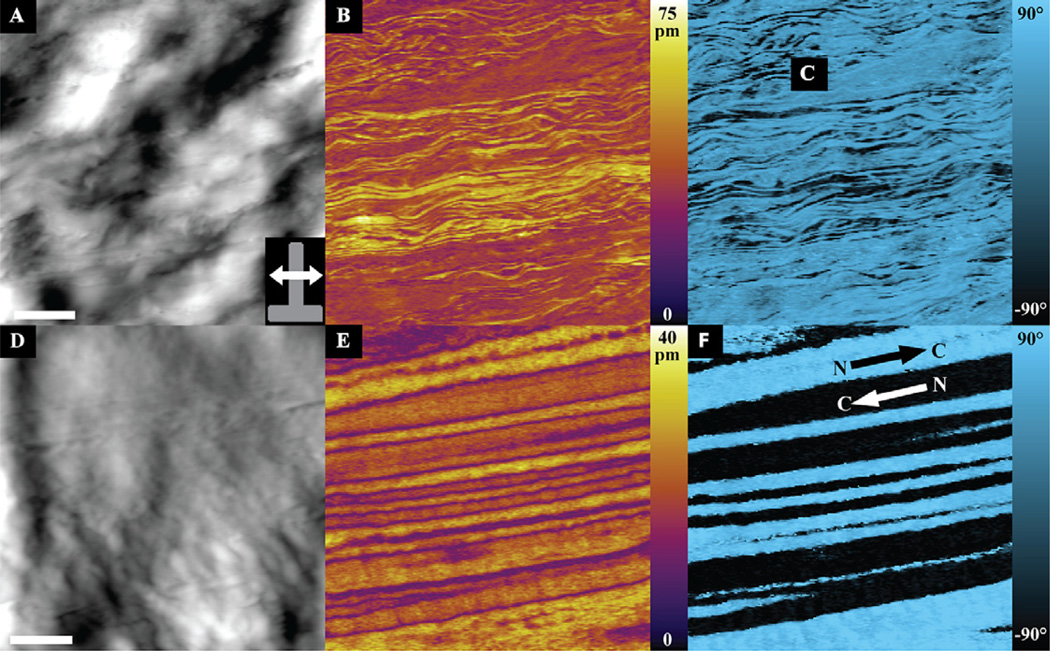
\includegraphics[scale=0.6]{PFM_コラーゲン_側面.jpg}
					\caption{コラーゲン繊維(側面)での面内PFM\cite{コラーゲン繊維PFM}.
					(A)AFM topology(B)面内PFM(C)面内PFMのPhase
					(D)AFM topology(E)面内PFM(F)面内PFMのPhase.
					(A)-(C)のスケールバーは2 {\textmu}m$\times$2 {\textmu}m, 
					(D)-(F)のスケールバーは200 nm$\times$200 nm.}
					\label{PFM_コラーゲン_側面}
					\end{center}
				\end{figure}
				\begin{figure}[h]
					\centering
					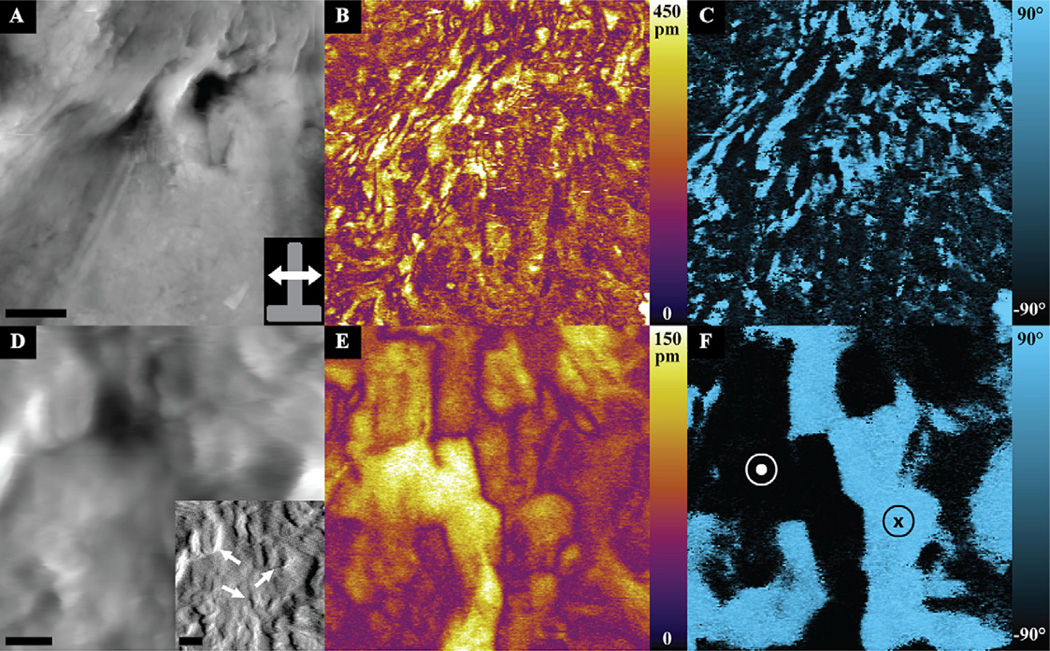
\includegraphics[scale=0.6]{PFM_コラーゲン_断面.jpg}
					\caption{コラーゲン繊維(断面)での垂直PFM\cite{コラーゲン繊維PFM}.
					(A)AFM topology(B)垂直PFM(C)垂直PFMのPhase
					(D)AFM topology(E)垂直PFM(F)垂直PFMのPhase.
					(A)-(C)のスケールバーは2 {\textmu}m $\times$ 2 {\textmu}m, 
					(D)-(F)のスケールバーは200 nm $\times$ 200 nm.}
					\label{PFM_コラーゲン_断面}
				\end{figure}
				\newpage
			\subsection{誘電率測定}
			\subsection{DSC}
	\chapter{結果と考察}
	\chapter{総括}
	\chapter{付録}
	\bibliography{master} %hoge.bibから拡張子を外した名前
	\bibliographystyle{junsrt} %参考文献出力スタイル
\end{document}